% \documentclass[12pt,a4paper]{report}
\documentclass[12pt,a4paper]{article}
\usepackage[utf8]{inputenc}
\usepackage[T1]{fontenc}
\usepackage{graphicx}
\usepackage{tikz}
\usetikzlibrary{positioning}
\usepackage{xcolor}
\usepackage{geometry}
\usepackage{hyperref}
\usepackage{enumitem}
\usepackage{booktabs}

\geometry{margin=1in}

\title{\textbf{Section X: Cybersecurity \& Cyber-Resilience Strategy for Sovereign Cloud/Edge Computing}}
\author{}
\date{}

\begin{document}

\maketitle

\tableofcontents
\newpage

\begin{figure}[h!]
		\centering
		\resizebox{\textwidth}{!}{%
		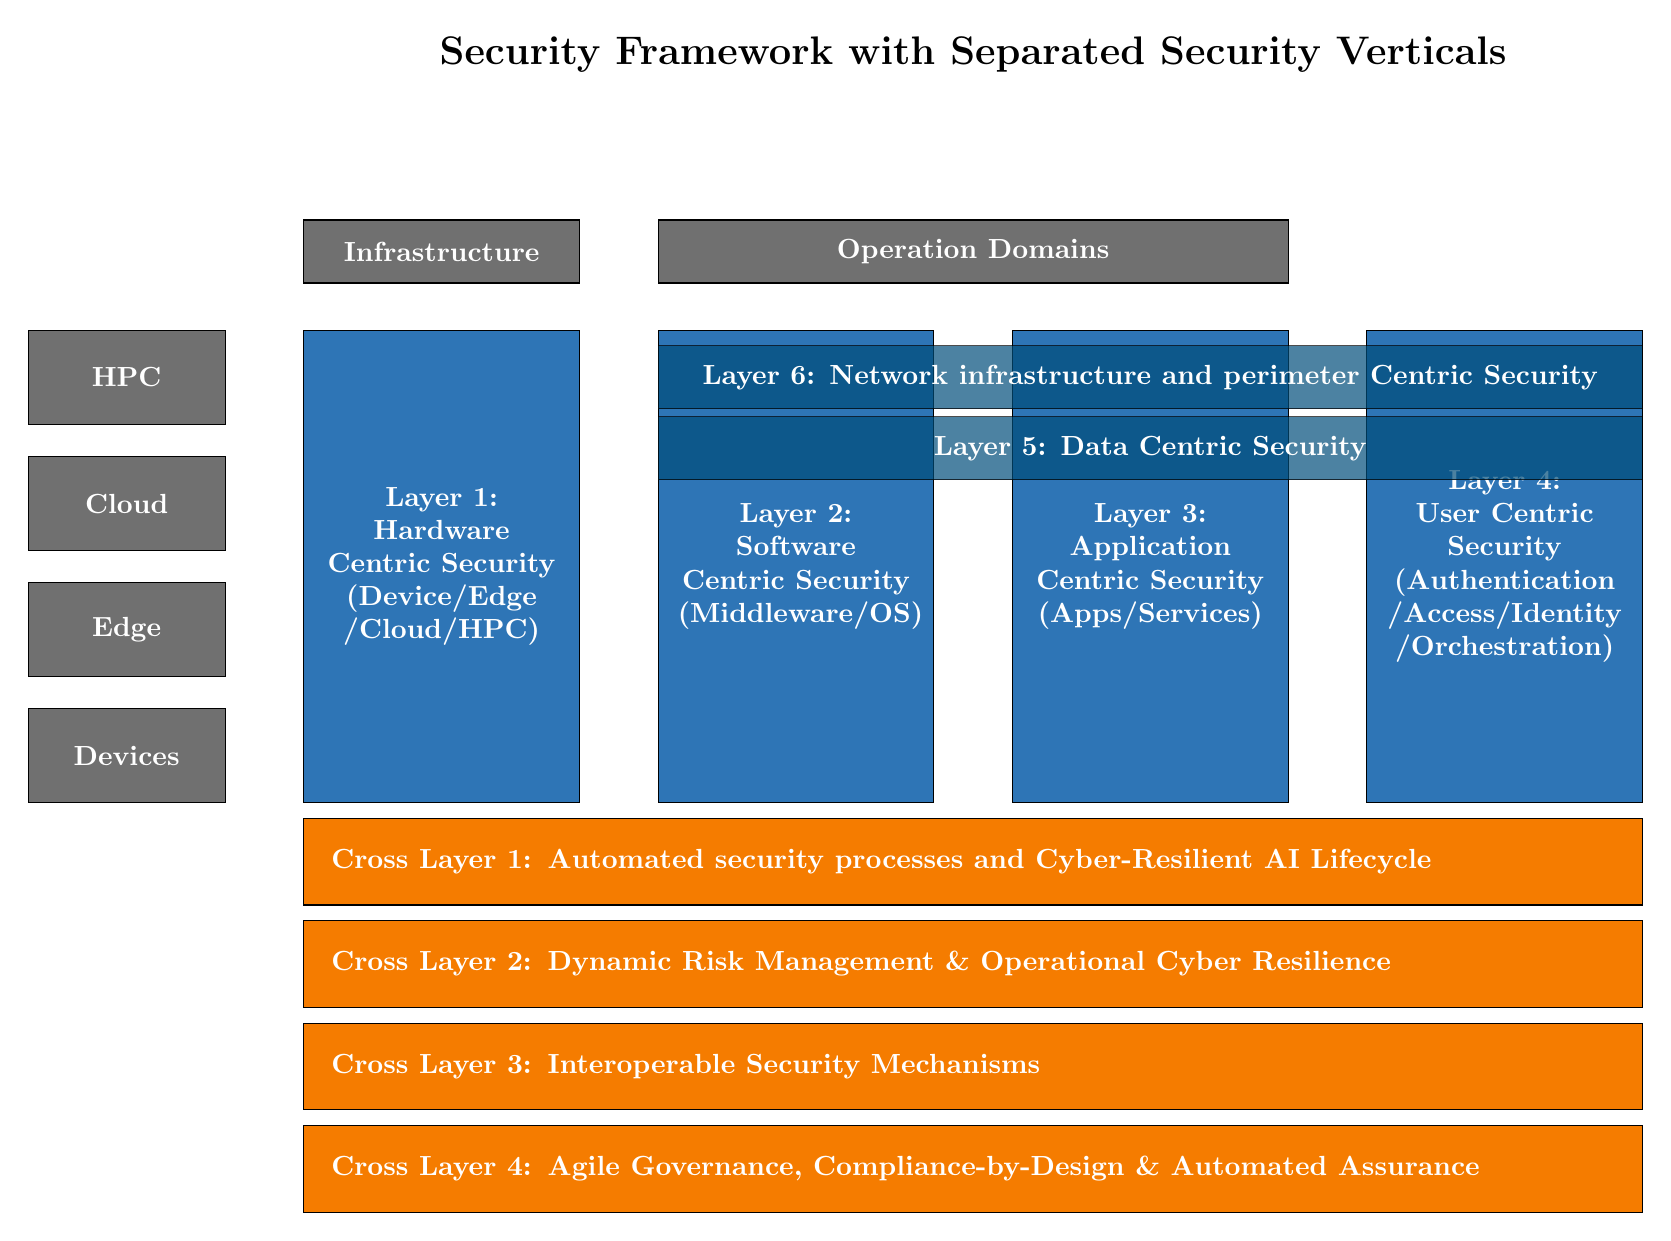
\begin{tikzpicture}[every node/.style={font=\small}]
			% Define colors
			\definecolor{archblue}{RGB}{46, 117, 182}
			\definecolor{sec_verticals_bg}{RGB}{245, 124, 0}
			\definecolor{env_bg}{RGB}{112, 112, 112}
			\definecolor{overlay}{RGB}{0, 77, 122}

			% Styles
			\tikzstyle{arch_col} = [fill=archblue, draw=black, text=white, font=\bfseries, minimum width=3.5cm, minimum height=6cm, align=center, text width=3cm]
			\tikzstyle{env_box} = [fill=env_bg, draw=black, text=white, font=\bfseries, minimum width=2.5cm, minimum height=1.2cm, align=center]
			\tikzstyle{top_tool} = [draw=black, fill=env_bg, text=white, minimum height=0.8cm, align=center, font=\bfseries]
			\tikzstyle{overlay_box} = [fill=overlay, draw=black, text=white, font=\bfseries, minimum height=0.8cm, align=center, opacity=0.7, text opacity=1]
			\tikzstyle{vertical_box} = [fill=sec_verticals_bg, draw=black, text=white, font=\bfseries, minimum width=17.0cm, minimum height=1.1cm, align=left, text width=16.3cm]

			% Column X positions
			\def\colone{-4.5}
			\def\coltwo{0}
			\def\colthree{4.5}
			\def\colfour{9}

			% Environment boxes (left)
			\node[env_box] at (-8.5, 2.4) {HPC};
			\node[env_box] at (-8.5, 0.8) {Cloud};
			\node[env_box] at (-8.5, -0.8) {Edge};
			\node[env_box] at (-8.5, -2.4) {Devices};

			% Main architecture columns representing layers
			\node[arch_col] (hw) at (\colone, 0) {Layer 1: \\ Hardware Centric Security \\ (Device/Edge\\ /Cloud/HPC)};
			\node[arch_col] (mw) at (\coltwo, 0) {Layer 2: \\ Software Centric Security \\ (Middleware/OS)};
			\node[arch_col] (app) at (\colthree, 0) {Layer 3: \\ Application Centric Security \\ (Apps/Services)};
			\node[arch_col] (user) at (\colfour, 0) {Layer 4: \\ User Centric Security \\ (Authentication\\ /Access/Identity\\ /Orchestration)};

			% Top tooling boxes
			\node[top_tool, minimum width=3.5cm] at (\colone, 4) {Infrastructure};
			\node[top_tool, minimum width=8cm] at (2.25, 4) {Operation Domains};

			% Arrows from tooling
			\draw[->, line width=2pt, white] (\colone, 3.5) -- (\colone, 3.1);
			\draw[->, line width=2pt, white] (2.25, 3.5) -- (2.25, 3.1);

			% Other layers as overlays/headers
			\node[overlay_box, minimum width=12.5cm] at (4.5, 1.5) {Layer 5: Data Centric Security};
			\node[overlay_box, minimum width=12.5cm] at (4.5, 2.4) {Layer 6: Network infrastructure and perimeter Centric Security};

			% Separated vertical boxes
			\node[vertical_box] at (2.25, -3.75) {\textbf{Cross Layer 1: Automated security processes and Cyber-Resilient AI Lifecycle}};
			\node[vertical_box] at (2.25, -5.05) {\textbf{Cross Layer 2: Dynamic Risk Management \& Operational Cyber Resilience}};
			\node[vertical_box] at (2.25, -6.35) {\textbf{Cross Layer 3: Interoperable Security Mechanisms}};
			\node[vertical_box] at (2.25, -7.65) {\textbf{Cross Layer 4: Agile Governance, Compliance-by-Design \& Automated Assurance}};

			% Title
			\node[font=\Large\bfseries, anchor=center] at (2.25, 6.5) {Security Framework with Separated Security Verticals};

		\end{tikzpicture}%
		}
		\caption{Security Framework with separated security verticals in dedicated boxes.}
		\label{fig:security_framework_verticals_boxes}
	\end{figure}

% \chapter{Structure and Instructions}
\noindent\textbf{Topic:} Cybersecurity for the Cognitive Computing Continuum\\
\textbf{Destinations:}
\begin{itemize}
    \item \textbf{Primary:} 4. A secure, sovereign European computing continuum infrastructure.
    \item \textbf{Secondary:} 6. European leadership in emerging disruptive computing paradigms.
\end{itemize}

\section{Background \& Driving Factors}
\begin{itemize}
    \item \textbf{Decentralization Risk:} The paradigm shift from the centralized Cloud to a distributed Cloud-Edge-IoT continuum radically expands the attack surface. This creates environments that are often ``too many, too diverse, and too dispersed'' to secure with traditional perimeter defenses.
    \item \textbf{Physical Exposure:} Edge nodes and far-edge IoT devices frequently operate in the field. Unlike hyperscaler data centers, they lack strict physical and environmental security controls, making them highly vulnerable to tampering.
    \item \textbf{Regulatory Pressure:} There is an immediate, complex need to operationalize the NIS2 Directive \cite{nis2}, the Cyber Resilience Act (CRA) \cite{cra}, and the AI Act \cite{aiact} across a highly fragmented technological ecosystem to ensure compliance and market access.
    \item \textbf{Digital Sovereignty:} Europe must urgently reduce its systemic reliance on non-EU technology providers. Doing so will mitigate extra-territorial data access risks and avoid geopolitical vendor lock-in, ensuring independent control over critical infrastructure.
\end{itemize}

\section{Europe in Relation to the State of the Art}
\textbf{Comparison vs. Hyperscalers:}
\begin{itemize}
    \item \textbf{EU Strengths:} Europe leads globally in Trust, Privacy-by-Design, proactive regulation (GDPR, Data Act, AI Act), and rigorous, standardized certification frameworks (e.g., EUCS \cite{eucs}).
    \item \textbf{EU Gaps:} The European market suffers from a lack of unified, hyper-scale security orchestration. Furthermore, there is a critical dependency on non-EU hardware (secure silicon) and highly fragmented threat intelligence sharing among member states.
\end{itemize}
\textbf{Strategic Goal:} To definitively transition the European computing continuum from a state of ``reactive, siloed security'' to an advanced architecture defined by ``autonomous, federated, and certified Security-by-Design.''

\section{Strategic Preamble}
\begin{itemize}
    \item \textbf{Context:} This section defines the architectural guardrails required to secure the Cloud-Edge-IoT Continuum. It moves beyond traditional ``perimeter security'' toward a model of Cyber-Resilience---where systems are engineered to proactively anticipate, withstand, recover from, and adapt to attacks while maintaining strict Digital Sovereignty.
    \item \textbf{Approach:} To provide actionable, risk-aware Research \& Innovation (R\&I) priorities, the strategy is organized into a two-part framework:
    \begin{itemize}
        \item \textbf{Capability Profiles (Qualitative):} A deep-dive 7-dimensional analysis defining exactly what needs to be built.
        \item \textbf{Progression Matrix (Quantitative \& Strategic):} A structured timeline tracking the evolution of capabilities through their Operational Deployment Phases and their trajectory toward Strategic Sovereignty.
    \end{itemize}
\end{itemize}

\section{The Core Capability Dimensions (Architectural Framework)}
As it is illustrated in Figure~\ref{fig:security_framework_verticals_boxes}, the roadmap is structured across a cohesive architectural framework that spans four continuum environments (HPC, Cloud, Edge, Devices). The capabilities are organized into Six Security Layers (The Vertical Stack) and Four Transversal Cross-Layers (The Horizontal Enablers).

\subsection*{Part A: The Security Layers (Vertical Stack)}
These layers define the specific technical security controls implemented across the computing infrastructure.

\subsubsection*{Layer 1: Hardware-Centric Security}
\textbf{1.1 Hardware Roots of Trust:} Cryptographically verifiable supply chain trust (e.g., TPM attestation, secure enclaves) ensures physical device integrity. Success depends on driving European open-hardware designs (e.g., RISC-V) toward \textbf{EUCC 'High' assurance level certification} \cite{eucc} to mathematically guarantee resistance against state-level physical tampering and side-channel attacks at the vulnerable far-edge.


\subsubsection*{Layer 2: Software-Centric Security (Middleware/OS)}
\textbf{2.1 OS \& Middleware Hardening:} Securing hypervisors, container runtimes, and distributed operating systems is critical for isolation. This involves hardening KVM/QEMU and supporting sovereign, lightweight Linux distributions optimized for edge resource constraints, ensuring a reduced attack surface for the cognitive continuum.

\subsubsection*{Layer 3: Application-Centric Security (Apps/Services)}
\textbf{3.1 Workload Security:} Securing containerized applications, microservices, and serverless functions executing dynamically across multi-provider nodes. This is achieved through hardened service meshes and sidecar proxy architectures that provide mutual TLS and granular traffic inspection without impacting performance.

\subsubsection*{Layer 4: User \& Orchestration-Centric Security}
\textbf{4.1 Zero-Trust Orchestration:} Seamless policy enforcement across a multi-provider computing continuum requires robust Policy Enforcement Point (PEP) and Policy Decision Point (PDP) architectures. This enables continuous authorization and dynamic access controls that adapt to the context of the request.

\textbf{4.2 Federated Identity \& Access Management (IAM):} Cross-domain identity federation and verifiable credentials for machines, users, and automated workloads. Implementing \textbf{Self-Sovereign Identity (SSI)} principles allows for cryptographically secure, decentralized authentication across heterogeneous cloud-edge domains.

\subsubsection*{Layer 5: Data-Centric Security}
\textbf{5.1 End-to-end Confidential Computing:} Data-in-use security through Trusted Execution Environments (TEEs) spanning the entire Cloud-to-IoT data path. Leveraging TEE abstraction layers and remote attestation ensures that sensitive European data remains encrypted even during processing in non-trusted environments.

\textbf{5.2 Post-Quantum \& Cryptographic Agility:} PQC standardization and hybrid crypto deployment are necessary to secure long-lived data. Priority is placed on \textbf{PQC migration for resource-constrained devices}, ensuring that edge infrastructure is resilient against "Harvest Now, Decrypt Later" quantum threats.

\subsubsection*{Layer 6: Network Infrastructure \& Perimeter-Centric Security}
\textbf{6.1 Telco-cloud \& O-RAN Security:} Hardening distributed 5G/6G cores and RAN components must align with the \textbf{Smart Networks and Services Joint Undertaking (SNS JU) SRIA} \cite{snsju}. This ensures sovereign control over network slice isolation and virtualized RAN components.

\textbf{6.2 Cross-Sector Physical Resilience \& Safety:} Adapting strict network controls and IT/OT gateway security for high-availability edge environments (e.g., Smart Grids). This guarantees that cyber-breaches in the digital layer do not cascade into physical safety hazards or kinetic damage in critical infrastructure.

\subsection*{Part B: The Transversal Security Verticals (Cross-Layers)}
These four cross-layers represent continuous, automated processes and governance structures that intersect every layer of the vertical stack.

\subsubsection*{Cross-Layer 1: Automated Security Processes \& Cyber-Resilient AI Lifecycle}
\textbf{CL1.1 Continuous DevSecOps (Shift-Left):} Embedding AI-driven code analysis and automated vulnerability remediation at the earliest stages of the software lifecycle.

\textbf{CL1.2 Model \& Pipeline Integrity (DataBOMs):} Securing AI training pipelines to prevent data poisoning and unauthorized model manipulation.

\textbf{CL1.3 Runtime AI Defense:} Defending AI/ML infrastructure against real-world adversarial attacks (e.g., prompt injection, model evasion/theft) at the edge.

\subsubsection*{Cross-Layer 2: Dynamic Risk Management \& Operational Cyber Resilience}
\textbf{CL2.1 Automated SOC Operations \& Collaborative Threat Intelligence:} Continuous monitoring, SOC federation across Member States, and automated incident containment, underpinned by legally protected, cross-border threat intelligence sharing ecosystems designed to overcome institutional trust barriers and incentivize active collaboration \cite{concordia}.

\textbf{CL2.2 Systemic \& Cascading Risk Mitigation:} Mapping the evolving threat landscape and using impact-likelihood scoring to dynamically sever links and prevent cross-domain systemic failures.

\subsubsection*{Cross-Layer 3: Interoperable Security Mechanisms \& Open-Source Verifiability}
\textbf{CL3.1 Heterogeneous Interoperability \& Simpl Integration:} Secure communication and data exchange across disparate systems, edge nodes, and proprietary domains. This includes mandatory alignment with and integration into the Simpl open-source smart middleware \cite{cloud_edge_roadmap} to ensure secure, federated access across Common European Data Spaces.

\textbf{CL3.2 Minimal Interoperability Mechanisms (MIMs) \& Open Verifiability:} Establishing standardized, baseline security and privacy controls to ensure trust without creating vendor lock-in. This relies heavily on embracing open-source software and open hardware architectures as fundamental prerequisites for transparency, cryptographic verifiability, and the elimination of proprietary black-box vulnerabilities \cite{cloud_edge_roadmap}.

\subsubsection*{Cross-Layer 4: Compliance-by-Design, Agile Governance \& Automated Assurance}
\textbf{CL4.1 Policy-as-Code \& Compliance-by-Design:} Technical implementation of legal requirements (OSCAL) into machine-readable rules that pre-validate workloads.

\textbf{CL4.2 Continuous Automated Auditing \& Certification Lifecycle:} Replacing ``point-in-time'' PDF certificates with real-time, telemetry-driven certification tracking for both cloud services (EUCS) \cite{eucs} and physical ICT edge products (EUCC) \cite{eucc}. This ensures that edge nodes autonomously maintain compliance by integrating mandatory vulnerability handling and cryptographic patch verification directly into their operational lifecycle, strictly aligning with EUCC maintenance and assurance rules \cite{eucc}.

\textbf{CL4.3 Regulatory Digital Twins:} Virtualized replicas of critical infrastructure specifically to stress-test regulatory compliance against evolving laws before applying changes to the live physical continuum.

\section{The 4-Filter Prioritization Framework}
To ensure the roadmap provides actionable guidance for European R\&I funding (Horizon Europe) and strategic investment, capabilities are prioritized using a structured 4-filter logic. This framework identifies the ``Critical Path'' items that require immediate resource allocation in Phase 1 (0-5 Yrs).

\begin{enumerate}
    \item \textbf{Regulatory Urgency (The ``Must-Do'' Filter):}
    \begin{itemize}
        \item \textbf{Question:} Is this capability strictly required to comply with imminent EU law (NIS2 \cite{nis2}, Cyber Resilience Act \cite{cra}, AI Act \cite{aiact})?
        \item \textbf{Logic:} If failure to achieve this by 2026 results in market exclusion or systemic non-compliance, it is designated as \textbf{Priority \#1}.
    \end{itemize}

    \item \textbf{Foundational Dependency (The ``Blocker'' Filter):}
    \begin{itemize}
        \item \textbf{Question:} Do subsequent security layers depend on this capability existing first?
        \item \textbf{Logic:} Foundational technologies (e.g., Layer 1 Hardware Trust) outrank high-level software orchestration. You cannot secure the user (Layer 4) if the hardware (Layer 1) cannot provide a verifiable anchor.
    \end{itemize}

    \item \textbf{The Sovereignty Cliff (The ``Extinction'' Filter):}
    \begin{itemize}
        \item \textbf{Question:} Does a lack of this tech pose an existential threat to EU sovereignty or systemic resilience?
        \item \textbf{Logic:} This prioritizes areas where the EU currently has 100\% foreign dependency or where a technical breakthrough (e.g., \textit{Q-Day} Quantum threat) would render existing defenses obsolete.
    \end{itemize}

    \item \textbf{Market Feasibility \& Ecosystem (The ``Simpl/SME'' Filter):}
    \begin{itemize}
        \item \textbf{Question:} Does this align with existing EU heavy-investments (e.g., Simpl \cite{cloud_edge_roadmap}) and is it adoptable by SMEs?
        \item \textbf{Logic:} Priority is given to capabilities that act as force-multipliers for existing infrastructure, ensuring economic viability.
    \end{itemize}
\end{enumerate}

\section*{Executive Priorities: The Critical Path (Phase 1)}
Applying the 4-Filter Framework, the following areas are identified as immediate strategic priorities for the 2025-2030 funding cycle:
\begin{itemize}
    \item \textbf{Priority 1:} Hardware Roots of Trust \& EUCC 'High' Certification (Filters 1, 2, 3).
    \item \textbf{Priority 2:} Post-Quantum Cryptographic Agility for Edge/IoT (Filter 3).
    \item \textbf{Priority 3:} Security Interoperability via Simpl Middleware (Filter 4).
\end{itemize}

\section{The Anatomy of a Roadmap Priorities: A 7-Dimensional Analysis}
To ensure the roadmap is actionable, realistic, and aligned with European strategic autonomy, every priority is analyzed holistically through a strict 7-point structural template:

\begin{enumerate}
    \item \textbf{Baseline \& Target Objective (The Trajectory) - Q: Where do we stand today, and what exactly does success look like?}\\
    \textit{Description:} Establishes the starting point of the priority today and defines the ultimate maturity state required by the end of the 15-year roadmap.
    \begin{itemize}
    \item \textbf{Baseline (Where we are):} Grounds the roadmap in reality. It captures the state of the art, current Operational Deployment Phase (ODP), Strategic Sovereignty Level (SSL), industrial capacity, reliance on foreign vendors, and the technical or economic barriers preventing immediate adoption.
    \item \textbf{Target (Where we need to be):} Sets the baseline for EU-funded projects, defining the target ODP and SSL that must be achieved by the end of the roadmap.
\end{itemize}
    
    \item \textbf{Primary Drivers (The ``Push'' Factors) - Q: Why must we prioritize building this capability right now? SQ: Why are we doing this?}\\
    \textit{Description:} Outlines the external pressures---both from the evolving threat landscape and mandatory EU regulations---that make this technological evolution urgent and unavoidable.
    \begin{itemize}
        \item \textbf{Threat Drivers:} The rapid advancement of adversarial capabilities (e.g., offensive AI, quantum decryption, supply chain targeting).
        \item \textbf{Regulatory Drivers:} Imminent EU compliance mandates that require technical operationalization (e.g., NIS2, Cyber Resilience Act, AI Act).
    \end{itemize}

    \item \textbf{High Impact Activities - Q: Which specific actions provide the greatest leap in European sovereignty and security? SQ: Which should be the key initiatives?}\\
    \textit{Description:} Highlights the specific, prioritized technical interventions within this broader capability group that will yield the highest strategic return on investment.

    \item \textbf{Catalysts \& Enablers (The ``Pull'' Factors \& EU Support) - Q: What specific EU funding, standards, and ecosystem support do we need? SQ: How do we get there \& accelerate?}\\
    \textit{Description:} Identifies the concrete mechanisms, funding vehicles, and regulatory standardizations required from the EU to accelerate market adoption and push the industry from the baseline to the target state.
    \begin{itemize}
        \item \textbf{R\&I \& Funding Alignment:} Required Horizon Europe funding topics and targeted innovation instruments. Investment priorities must be explicitly synchronized with the European Cybersecurity Competence Centre (ECCC) Strategic Agenda \cite{eccc} to ensure alignment with pan-European goals (e.g., PQC transition infrastructure, AI-driven security tools).
        \item \textbf{Regulatory \& Standardization:} Alignment with standard-setting bodies (CEN/CENELEC) and certification frameworks (e.g., EUCS, EUCC).
        \item \textbf{Ecosystem:} Support for ecosystem building, industrial partnerships, and capacity-building initiatives (e.g., federated Cyber Ranges) to upskill the workforce and ensure advanced security solutions are economically viable for SMEs.
    \end{itemize}

    \item \textbf{Disruptors \& Systemic Risks (The Roadblocks) - Q: What structural vulnerabilities, market failures, or adversary breakthroughs could derail us? SQ: What can break the path?}\\
    \textit{Description:} Acknowledges that innovation is not linear by identifying severe technical and architectural risks that could actively derail deployment. It places primary emphasis on ``Technical Cliffs''---moments where defensive capabilities are rendered obsolete by adversarial breakthroughs before countermeasures are fully deployed.
    \begin{itemize}
        \item \textbf{Cryptographic Obsolescence \& Migration Bottlenecks (The Primary Technical Risk):}
        \begin{itemize}
            \item \textit{The ``Q-Day'' Cliff:} The risk that Cryptographically Relevant Quantum Computers (CRQC) become operational before the EU completes its migration to Post-Quantum Cryptography (PQC). This creates a ``Harvest Now, Decrypt Later'' vulnerability.
            \item \textit{Migration Complexity:} The systemic failure to inventory and replace deep-rooted Public Key Infrastructure (PKI) in legacy OT/IoT environments.
        \end{itemize}
        \item \textbf{Adversarial Breakthroughs:} The risk of threat actors weaponizing emerging technologies (e.g., AI-driven exploit generation, polymorphic malware) faster than defensive R\&I can mitigate them.
        \item \textbf{Contextual Risks (Non-Technical / Optional):} Geopolitics \& Supply Chain dependencies, Market \& Tech Risks (monopolization, fragmented standards).
    \end{itemize}

    \item \textbf{Failsafe Mechanisms \& Resilience (The Safety Nets) - Q: If this technology is compromised, how does the system survive and gracefully degrade? SQ: How do we prevent failure?}\\
    \textit{Description:} The technical core of ``Cyber-Resilience.'' It defines the engineering fallbacks required if a primary capability fails, is breached, or is disrupted by the systemic risks identified above.\\
    \textbf{What it entails:} Designing for degraded modes of operation, architectural redundancies, autonomous isolation protocols, and implementation diversity to avoid vulnerable technological monocultures.

    \item \textbf{Transversal Meta-Layer (The Policy Alignment) - Q: How does mastering this capability support Europe's goals of sovereignty, sustainability, and trust? SQ: The broader policy context?}\\
    \textit{Description:} Elevates the technical capability back to the overarching political and societal goals of the European Union.
    \begin{itemize}
        \item \textbf{Sovereignty \& Autonomy:} Strengthening European strategic independence, reducing reliance on non-EU vendors.
        \item \textbf{Trust \& Ethics:} Fostering deep Societal Trust by guaranteeing data privacy (Privacy-by-Design), algorithmic fairness, and transparency.
        \item \textbf{Sustainable Security (Green IT):} Minimizing the environmental impact of cyber defense (e.g., energy-efficient cryptographic algorithms, crypto-agility to reduce e-waste).
    \end{itemize}
\end{enumerate}

\section{Progression Matrix: Sequence of Events (X-Axis)}
Instead of a strictly chronological timeline, the roadmap maps the sequence of critical events required to unlock maturity. This ensures that foundational capabilities are built before advanced autonomous systems.

\begin{itemize}
    \item \textbf{Phase 1: Foundation \& Compliance (Immediate Implementation):} Focuses on state-of-practice deployments, bridging immediate capability gaps, and addressing urgent regulatory obligations (NIS2, CRA).
    \item \textbf{Phase 2: Federation \& Standardization (Scaling \& Harmonization):} Focuses on deploying emerging technologies, establishing harmonized governance frameworks, and managing critical transition periods.
    \item \textbf{Phase 3: Autonomy \& Leadership (Sovereign Innovation):} Focuses on highly speculative but structured foresight, including defense against quantum-capable adversaries and the achievement of fully sovereign, autonomous cloud-edge ecosystems.
\end{itemize}

\subsection*{Matrix Cell Content Definition (Measuring Progression)}
Rather than relying on subjective Technology Readiness Levels (TRL) or Manufacturing Readiness Levels (MRL) for a highly fragmented ecosystem, each cell in the progression matrix tracks maturity using objective strategic market and policy indicators:

\begin{itemize}
    \item \textbf{Operational Deployment Phase (ODP):} Tracks the market reality and integration status (e.g., \textit{Applied R\&D $\rightarrow$ Fragmented Piloting $\rightarrow$ Standardized Integration $\rightarrow$ Ubiquitous Operation}).
    \item \textbf{Strategic Sovereignty Level (SSL):} Tracks European strategic autonomy and reliance on foreign vendors (e.g., \textit{High Foreign Dependency $\rightarrow$ Emerging EU Ecosystem $\rightarrow$ Full Sovereign Autonomy}).
    \item \textbf{Operational State:} A concise snapshot characterizing the reality on the ground during this phase.
    \item \textbf{Critical Enabler:} The single most critical regulation, standard, or European R\&I breakthrough unlocking the transition to the next phase.
\end{itemize}

\newpage
% =========================================================================
% CHAPTER 1: INSTRUCTIONS
% =========================================================================
\section{Chapter 1: Instructions for Using This Roadmap Framework}

\subsection*{Purpose of This Document}
This roadmap provides a structured methodology for European policymakers, research organizations, and industry stakeholders to:
\begin{itemize}
    \item Identify and prioritize cybersecurity R\&I investments for the Cloud-Edge-IoT continuum
    \item Track capability maturity using objective Operational Deployment Phase (ODP) and Strategic Sovereignty Level (SSL) metrics
    \item Align Horizon Europe funding with strategic autonomy goals and regulatory compliance requirements
    \item Ensure coordinated implementation across Member States and European initiatives (ECCC, Digital Europe Programme, EU Chips Act)
\end{itemize}

\subsection*{Target Audiences}
\begin{description}
    \item[European Commission \& Funding Bodies:] Use the 4-Filter Prioritization Framework to allocate Horizon Europe, Digital Europe Programme, and ECCC funding to capabilities with the highest strategic impact.
    
    \item[National Cybersecurity Agencies:] Leverage the progression matrices to coordinate national R\&I investments with EU-wide timelines and ensure interoperability across Member States.
    
    \item[Research Consortia \& Industry:] Utilize the 7-Dimensional Analysis template to structure project proposals, clearly articulating baseline, target, drivers, risks, and alignment with European strategic goals.
    
    \item[Standardization Bodies (CEN/CENELEC, ETSI):] Reference the architectural framework and MIMs to develop harmonized standards for secure, interoperable computing continuum infrastructure.
\end{description}

\subsection*{How to Navigate This Document}
\begin{enumerate}
    \item \textbf{Start with Section 1-3:} Understand the threat landscape, regulatory drivers, and strategic context for securing the European computing continuum.
    
    \item \textbf{Review Section 4:} Familiarize yourself with the 6 Security Layers and 4 Cross-Layers comprising the architectural framework.
    
    \item \textbf{Apply Section 5:} Use the 4-Filter Prioritization Framework to assess which capabilities are critical for your specific context (national strategy, industrial sector, research focus).
    
    \item \textbf{Study Section 6-7:} Understand the 7-Dimensional Analysis methodology and ODP/SSL progression metrics before designing projects or policies.
    
    \item \textbf{Reference Section 9 (Priorities 1-3):} Use the detailed capability profiles as templates for structuring additional priorities relevant to your domain.
    
    \item \textbf{Implement Section 10:} Actionable strategic recommendations for Phase 1 (2025-2030) provide concrete next steps.
\end{enumerate}

\subsection*{Key Principles}
\begin{itemize}
    \item \textbf{Evidence-Based Prioritization:} All priorities must pass the 4-Filter Framework (Regulatory Urgency, Foundational Dependency, Sovereignty Cliff, Market Feasibility).
    
    \item \textbf{Sovereignty-First Design:} Investments should systematically reduce foreign dependencies (measured via SSL metrics) while building European industrial capacity.
    
    \item \textbf{Compliance-by-Design:} All R\&I outputs must align with or anticipate NIS2, CRA, AI Act, and Data Act requirements to ensure market relevance.
    
    \item \textbf{Federated Interoperability:} Solutions must prioritize standardization and open architectures (e.g., Simpl middleware, open-source RISC-V) over proprietary, siloed approaches.
    
    \item \textbf{Measurable Progression:} Avoid subjective TRL assessments; instead, use objective ODP (market integration) and SSL (sovereignty) metrics with clear phase transition criteria.
\end{itemize}

\newpage
% =========================================================================
% CHAPTER 2: PROMPT
% =========================================================================
\section{Chapter 2: Master Prompt for Generating Capability Profiles}

\subsection*{Context for Content Generation}
You are an expert EU Cybersecurity Policy Strategist and Technical Architect. Your task is to populate capability profiles for the European Cloud-Edge-IoT Cybersecurity Roadmap using the structured framework defined in this document. Each capability profile must be rigorously aligned with European strategic autonomy goals, regulatory requirements, and the specific needs of the distributed computing continuum.

\subsection*{Input Requirements}
Before generating a capability profile, ensure you have:
\begin{itemize}
    \item \textbf{Capability Name:} Clear, concise identifier (e.g., ``Zero-Trust Network Architecture for Edge'')
    \item \textbf{Architectural Placement:} Which Layer(s) or Cross-Layer(s) does this capability belong to? (Refer to Section 4)
    \item \textbf{Priority Justification:} Which filters from the 4-Filter Framework does this capability satisfy? (Section 5)
    \item \textbf{Contextual Scope:} Is this capability specific to HPC, Cloud, Edge, or Devices? Or does it span multiple environments?
\end{itemize}

\subsection*{Generation Template: 7-Dimensional Analysis}
For each capability, generate a complete analysis following this exact structure:

\subsubsection*{Dimension 1: Baseline \& Target Objective}
\begin{itemize}
    \item \textbf{Baseline (Current State):} Describe the state of the art in Europe as of 2025-2026. Include:
    \begin{itemize}
        \item Current ODP level (Applied R\&D / Fragmented Piloting / Standardized Integration)
        \item Current SSL level (High Foreign Dependency / Emerging EU Ecosystem / Full Sovereign Autonomy)
        \item Specific technical/economic barriers preventing immediate adoption
        \item Market fragmentation or vendor lock-in issues
    \end{itemize}
    \item \textbf{Target (Desired State by 2040):} Define success. Include:
    \begin{itemize}
        \item Target ODP: Ubiquitous Operation across the continuum
        \item Target SSL: Full Sovereign Autonomy with quantified EU market share (e.g., ``60\% of edge secure elements are EU-designed'')
        \item Measurable technical outcomes (e.g., ``100\% of critical IoT devices support PQC'')
    \end{itemize}
\end{itemize}

\subsubsection*{Dimension 2: Primary Drivers}
\begin{itemize}
    \item \textbf{Threat Drivers:} What adversarial capabilities or attack vectors make this urgent?
    \begin{itemize}
        \item Examples: Side-channel attacks on edge TPMs, quantum decryption threats, AI-driven exploit automation
    \end{itemize}
    \item \textbf{Regulatory Drivers:} Which EU laws mandate or incentivize this capability?
    \begin{itemize}
        \item Cite specific directives: NIS2 Article X, CRA Annex Y, AI Act requirements
        \item Include enforcement timelines (e.g., ``NIS2 full enforcement by October 2024'')
    \end{itemize}
\end{itemize}

\subsubsection*{Dimension 3: High Impact Activities}
List 3-5 specific technical interventions that will yield the greatest strategic ROI:
\begin{itemize}
    \item Be concrete: ``Develop automated TEE attestation for heterogeneous edge fleets'' (not ``Improve edge security'')
    \item Prioritize activities that unlock multiple downstream capabilities
    \item Indicate which activities target Phase 1 vs. Phase 2-3
\end{itemize}

\subsubsection*{Dimension 4: Catalysts \& Enablers}
\begin{itemize}
    \item \textbf{Funding Alignment:} Which Horizon Europe clusters, Digital Europe Programme calls, or ECCC work packages should fund this? Reference the \textbf{ECCC Strategic Agenda} explicitly.
    \item \textbf{Standardization:} Which CEN/CENELEC, ETSI, or ISO standards are required? Are they existing or need development?
    \item \textbf{Ecosystem Enablers:} Pilot infrastructure (e.g., federated Cyber Ranges), industry partnerships (e.g., Gaia-X integration), SME support schemes.
\end{itemize}

\subsubsection*{Dimension 5: Disruptors \& Systemic Risks}
Identify severe risks that could derail the roadmap:
\begin{itemize}
    \item \textbf{Technical Cliffs:} Examples: Q-Day arriving before PQC migration; breakthrough in TEE side-channel attacks rendering current enclaves obsolete
    \item \textbf{Market \& Supply Chain:} Examples: EU Chips Act fabrication delays; vendor resistance to open standards; monopolization by non-EU providers
    \item \textbf{Geopolitical:} Examples: Export controls on critical components; extra-territorial jurisdiction conflicts
\end{itemize}

\subsubsection*{Dimension 6: Failsafe Mechanisms \& Resilience}
Define engineering fallbacks if the primary capability fails:
\begin{itemize}
    \item \textbf{Redundancy:} Hybrid approaches (e.g., classical + PQC crypto during transition)
    \item \textbf{Graceful Degradation:} How does the system continue operating in a compromised state?
    \item \textbf{Autonomous Isolation:} Automated quarantine protocols for compromised nodes
    \item \textbf{Implementation Diversity:} Avoid monocultures (e.g., deploy multiple TEE technologies, not just one vendor)
\end{itemize}

\subsubsection*{Dimension 7: Transversal Meta-Layer}
Connect the technical capability to overarching EU policy goals:
\begin{itemize}
    \item \textbf{Sovereignty \& Autonomy:} How does this reduce extra-territorial dependencies?
    \item \textbf{Trust \& Ethics:} How does this uphold GDPR principles, Privacy-by-Design, algorithmic transparency?
    \item \textbf{Sustainability (Green IT):} Energy efficiency, e-waste reduction, circular economy alignment
\end{itemize}

\subsection*{Generation Template: Progression Matrix}
After completing the 7-Dimensional Analysis, generate a progression matrix with this structure:

\begin{itemize}
    \item \textbf{Row 1 - ODP:} Applied R\&D $\rightarrow$ Fragmented Piloting $\rightarrow$ Standardized Integration $\rightarrow$ Ubiquitous Operation
    \item \textbf{Row 2 - SSL:} High Foreign Dependency $\rightarrow$ Emerging EU Ecosystem $\rightarrow$ Full Sovereign Autonomy
    \item \textbf{Row 3 - Operational State:} 2-3 sentence snapshot of ``what's happening on the ground'' in this phase
    \item \textbf{Row 4 - Critical Enabler:} The single most important regulation, standard, or R\&I breakthrough required to transition to the next phase
\end{itemize}

\subsection*{Mandatory Integration Points}
All generated profiles MUST reference:
\begin{itemize}
    \item \textbf{Simpl Middleware:} If the capability involves cross-provider interoperability or Data Spaces (CL3.1)
    \item \textbf{SNS JU SRIA:} If the capability involves 5G/6G, network slicing, or telco-cloud (Layer 6.1)
    \item \textbf{EUCS/EUCC:} If the capability involves certification, compliance automation, or assurance (CL4.2)
    \item \textbf{ECCC Strategic Agenda:} All profiles must align funding recommendations with ECCC priorities
\end{itemize}

\subsection*{Tone \& Style Requirements}
\begin{itemize}
    \item \textbf{Evaluator-Grade Rigor:} Assume the audience includes European Commission evaluators, national cybersecurity directors, and technical auditors
    \item \textbf{Actionable Specificity:} Avoid generic statements; provide concrete activities, timelines, and funding mechanisms
    \item \textbf{Evidence-Based:} Cite regulations, standardization efforts, and existing EU initiatives
    \item \textbf{Balanced Realism:} Acknowledge risks and uncertainties; avoid over-promising on speculative technologies
\end{itemize}

\newpage
% =========================================================================
% CHAPTER 3: EXECUTION
% =========================================================================
\section{Chapter 3: Execution Roadmap for Implementation}

\subsection*{Overview}
This chapter provides a step-by-step execution framework for translating the strategic priorities identified in this roadmap into actionable R\&I projects, policy measures, and industrial deployments across the 2025-2040 timeline.

\subsection*{Phase 1: Foundation \& Compliance (2025-2030)}

\subsubsection*{Year 1-2 (2025-2026): Strategic Alignment \& Pilot Initiation}
\textbf{Policy \& Governance Actions:}
\begin{itemize}
    \item Establish inter-DG coordination mechanism (DG CONNECT, DG CNECT, ECCC) for unified cybersecurity investment strategy
    \item Finalize and publish EU-wide PQC migration guidelines (ENISA lead)
    \item Launch Simpl Governance Board with security workstream mandate
    \item Issue Horizon Europe calls explicitly aligned with Priority 1-3 (Hardware RoT, PQC, Simpl)
\end{itemize}

\textbf{R\&I \& Technology Actions:}
\begin{itemize}
    \item Fund 3-5 RISC-V secure element pilot projects targeting EUCC 'High' certification
    \item Initiate PQC optimization research for 8/16-bit microcontrollers (embedded systems focus)
    \item Deploy Simpl security MIM pilots in 2-3 Data Spaces (e.g., Manufacturing, Health)
    \item Establish federated Cyber Range infrastructure for cross-border SOC training
\end{itemize}

\textbf{Success Metrics:}
\begin{itemize}
    \item At least 50M EUR allocated to sovereign secure silicon R\&D
    \item ENISA PQC guidelines published and adopted by 5+ Member States
    \item 2+ Common Data Spaces operationally testing Simpl security modules
\end{itemize}

\subsubsection*{Year 3-4 (2027-2028): Standardization \& Scale-Up}
\textbf{Policy \& Governance Actions:}
\begin{itemize}
    \item Enforce CRA compliance verification for all new IoT/edge products entering EU market
    \item Publish CEN/CENELEC standards for security MIMs and crypto-agility frameworks
    \item Establish continuous certification pilot programs for EUCS/EUCC (replace point-in-time audits)
    \item Launch EU Chips Act secure silicon fabrication pilot lines
\end{itemize}

\textbf{R\&I \& Technology Actions:}
\begin{itemize}
    \item Transition RISC-V secure elements from TRL 6-7 to industrial production (TRL 8-9)
    \item Deploy hybrid PQC schemes in critical infrastructure (energy grids, financial systems)
    \item Scale Simpl-based security across 50\%+ of active Common Data Spaces
    \item Operationalize automated SOC federation with cross-border threat intelligence sharing (CONCORDIA successor)
\end{itemize}

\textbf{Success Metrics:}
\begin{itemize}
    \item First EU-manufactured EUCC 'High' certified secure elements in production
    \item 30\% of new critical IoT deployments support hybrid (classical + PQC) cryptography
    \item Simpl security MIMs adopted as official CEN standard
\end{itemize}

\subsubsection*{Year 5 (2029-2030): Market Penetration \& Assessment}
\textbf{Policy \& Governance Actions:}
\begin{itemize}
    \item Conduct comprehensive Phase 1 evaluation against 2030 success metrics (Section 10)
    \item Issue Phase 2 funding strategy based on Phase 1 outcomes and emerging threats
    \item Mandate PQC support for all new public sector ICT procurement
\end{itemize}

\textbf{R\&I \& Technology Actions:}
\begin{itemize}
    \item Achieve 30\%+ market share for EU secure silicon in critical edge infrastructure
    \item Complete cryptographic inventory of 80\%+ legacy OT/IoT systems (PQC migration readiness)
    \item Demonstrate fully automated, real-time EUCS/EUCC certification tracking in operational Data Space
\end{itemize}

\textbf{Success Metrics:}
\begin{itemize}
    \item SSL metric: Transition from ``High Foreign Dependency'' to ``Emerging EU Ecosystem'' for Priority 1
    \item ODP metric: Transition from ``Fragmented Piloting'' to ``Standardized Integration'' for Priorities 2-3
\end{itemize}

\subsection*{Phase 2: Federation \& Standardization (2030-2035)}

\subsubsection*{Strategic Focus Areas}
\begin{itemize}
    \item \textbf{Quantum-Resilient Continuum:} Complete PQC migration for all critical infrastructure; deprecate classical-only cryptography in high-security contexts
    \item \textbf{Autonomous Security Orchestration:} Deploy AI-driven, zero-trust policy enforcement across federated Cloud-Edge ecosystems
    \item \textbf{European Certification Fabric:} Ubiquitous continuous certification with automated compliance verification for NIS2/CRA/AI Act
    \item \textbf{Sovereign Supply Chains:} Achieve 60\%+ EU market share for secure silicon; establish resilient fabrication capacity
\end{itemize}

\subsubsection*{Key Execution Milestones}
\begin{itemize}
    \item 2031: NIST PQC algorithm finalization triggers mandatory adoption timelines
    \item 2032: EU-wide deployment of PQC-native RISC-V processors in new edge infrastructure
    \item 2033: Simpl-based security standard becomes mandatory for all EU-funded cloud/edge projects
    \item 2034: First ``Quantum-Safe Data Space'' fully operational with end-to-end PQC
    \item 2035: Phase 2 completion assessment; 70\%+ Data Spaces using automated policy federation
\end{itemize}

\subsection*{Phase 3: Autonomy \& Leadership (2035-2040)}

\subsubsection*{Strategic Vision}
Establish Europe as the global leader in secure, sovereign, and sustainable computing continuum infrastructure. Achieve:
\begin{itemize}
    \item \textbf{Full Sovereign Autonomy (SSL):} EU-designed security components dominate European market; zero critical dependencies on extra-territorial providers
    \item \textbf{Ubiquitous Operation (ODP):} Security-by-Design is the default; manual security configuration is obsolete
    \item \textbf{Export Leadership:} European cybersecurity standards and technologies become global reference implementations
\end{itemize}

\subsubsection*{Key Execution Milestones}
\begin{itemize}
    \item 2036: European ``Quantum-Native'' computing continuum fully operational
    \item 2037: 100\% of EU Common Data Spaces operate on provider-agnostic, zero-trust architectures
    \item 2038: Continuous automated certification becomes global best practice (EU-led standardization)
    \item 2039: EU Chips Act sovereign fabrication meets 80\%+ of European secure silicon demand
    \item 2040: Roadmap completion assessment; initiate next-generation strategy for post-quantum, neuromorphic, and space-based edge computing security
\end{itemize}

\subsection*{Cross-Phase Execution Principles}

\subsubsection*{Continuous Monitoring \& Adaptation}
\begin{itemize}
    \item \textbf{Annual Reviews:} ECCC-led assessment of ODP/SSL progression against roadmap targets
    \item \textbf{Threat Landscape Updates:} Quarterly intelligence briefs on emerging attack vectors requiring roadmap adjustments
    \item \textbf{Technology Watch:} Monitor adversarial R\&I (e.g., quantum computing breakthroughs) and adjust timelines accordingly
\end{itemize}

\subsubsection*{Stakeholder Coordination}
\begin{itemize}
    \item \textbf{Public-Private Partnerships:} Formalize collaboration frameworks between ECCC, national agencies, and industry consortia
    \item \textbf{SME Inclusion:} Dedicated support programs ensuring SMEs can participate without discriminatory certification/compliance costs
    \item \textbf{Academic Integration:} Align university curricula with roadmap skill requirements (PQC, TEE development, federated security)
\end{itemize}

\subsubsection*{Risk Mitigation \& Resilience}
\begin{itemize}
    \item \textbf{Failfast Protocols:} Quarterly ``red team'' assessments of roadmap assumptions; rapid pivot mechanisms if technologies fail to mature
    \item \textbf{Geopolitical Hedging:} Diversified supply chains; strategic stockpiles of critical components
    \item \textbf{Implementation Diversity:} Avoid betting on single technologies; maintain parallel development tracks for critical capabilities
\end{itemize}


% =========================================================================
% CONTENT GENERATION AREA (The actual capability profiles will go here)
% =========================================================================
\newpage
\section{Capability Profiles \& Progression Matrices}

% --- TEMPLATE FOR CAPABILITY PROGRESSION MATRIX ---
\vspace{0.5cm}
\noindent\textbf{Progression Matrix: [Insert Capability Name]}
\vspace{0.2cm}

\noindent
\resizebox{\textwidth}{!}{%
\begin{tabular}{|p{3cm}|p{4.5cm}|p{4.5cm}|p{4.5cm}|}
\hline
\textbf{Metric} & \textbf{Phase 1: Foundation \& Compliance (0-5 Yrs)} & \textbf{Phase 2: Federation \& Standardization (5-10 Yrs)} & \textbf{Phase 3: Autonomy \& Leadership (10-15 Yrs)} \\ \hline
\textbf{Deployment Phase (ODP)} & Fragmented Piloting & Standardized Integration & Ubiquitous Operation \\ \hline
\textbf{Sovereignty Level (SSL)} & High Foreign Dependency & Emerging EU Ecosystem & Full Sovereign Autonomy \\ \hline
\textbf{Operational State} & [Cloud vs Edge snapshot here] & [Cloud vs Edge snapshot here] & [Cloud vs Edge snapshot here] \\ \hline
\textbf{Critical Enabler} & [Regulation/Standard here] & [Standard/Funding here] & [Autonomy milestone here] \\ \hline
\end{tabular}%
}
\vspace{0.5cm}


% =========================================================================
% MASTER PROMPT
% =========================================================================
\section{Master Population Prompt for Roadmap Generation}

\noindent\textbf{Context:} You are an expert EU Cybersecurity Policy Strategist. Your task is to populate the content for a Horizon Europe roadmap document based on the provided Master LaTeX structure.

\subsection*{Phase 1: Populate Section 4 (Architectural Summaries)}
Using a \texttt{description} environment, provide a 2-3 sentence strategic summary for every Layer and Cross-Layer. 
\begin{itemize}
    \item \textbf{Layers 1--6:} Connect the technical component to its role in the continuum.
    \item \textbf{Cross-Layers 1--4:} Emphasize automation and governance.
    \item \textbf{Mandatory Hooks:} Reference \textbf{SNS JU SRIA} in 6.1, \textbf{Simpl Middleware} and \textbf{Common European Data Spaces} in CL3.1, and \textbf{EUCS/EUCC} in CL4.2.
\end{itemize}

\subsection*{Phase 2: Priority Selection \& 7-Dimensional Analysis}
Apply the \textbf{4-Filter Prioritization Framework} (Regulatory Urgency, Foundational Dependency, Sovereignty Cliff, and Market Feasibility) to justify the selection of the Top 3 Priorities:
\begin{enumerate}
    \item \textbf{Priority 1:} Hardware Roots of Trust \& EUCC 'High' Certification.
    \item \textbf{Priority 2:} Post-Quantum Cryptographic (PQC) Agility for Edge/IoT.
    \item \textbf{Priority 3:} Security Interoperability via Simpl Middleware.
\end{enumerate}
For each priority, generate a full analysis using the \textbf{7-Dimensional Template} (Baseline/Target, Drivers, High Impact Activities, Catalysts/ECCC, Disruptors/Q-Day, Failsafe, and Policy Meta-Layer).

\subsection*{Phase 3: Progression Matrices}
Generate a LaTeX \texttt{tabular} matrix for each priority using the \textbf{ODP} (Operational Deployment Phase) and \textbf{SSL} (Strategic Sovereignty Level) metrics across the three time horizons.
\begin{itemize}
    \item \textbf{Phase 1 (0-5 Yrs):} Target NIS2/CRA compliance and bridging foreign dependency.
    \item \textbf{Phase 2 (5-10 Yrs):} Focus on standardized federation and EU-wide certification.
    \item \textbf{Phase 3 (10-15 Yrs):} Achieve full sovereign autonomy and quantum-native resilience.
\end{itemize}

\noindent\textbf{Tone \& Style:} Evaluator-grade, formal, and strictly aligned with the \textit{European Industrial Technology Roadmap for the Next-Generation Cloud-Edge}.


\section{The Core Capability Dimensions (Architectural Framework)}
The roadmap is structured across a cohesive architectural framework that spans four continuum environments (HPC, Cloud, Edge, Devices).

\subsection*{Part A: The Security Layers (Vertical Stack)}
\begin{description}
\item[Layer 1.1 Hardware Roots of Trust:] Cryptographically verifiable supply chain trust ensures physical device integrity from fabrication to deployment. Success depends on driving European open-hardware designs (e.g., RISC-V) toward \textbf{EUCC 'High' assurance} certification \cite{eucc} to guarantee resistance against state-level physical tampering at the vulnerable far-edge.

\item[Layer 2.1 OS \& Middleware Hardening:] Securing hypervisors and distributed operating systems across the continuum. This involves hardening KVM/QEMU and supporting sovereign, lightweight Linux distributions optimized for edge resource constraints, ensuring a minimal attack surface for cognitive workloads.

\item[Layer 3.1 Workload Security:] Securing containerized applications and serverless functions executing dynamically across multi-provider nodes. Implementation of hardened service meshes and sidecar proxy architectures provides mutual TLS and granular traffic inspection without impacting performance.

\item[Layer 4.1 Zero-Trust Orchestration:] Seamless policy enforcement across a multi-provider computing continuum requiring robust PEP/PDP architectures. This enables continuous authorization and dynamic access controls that adapt to the specific context of the request.

\item[Layer 4.2 Federated Identity \& Access Management (IAM):] Cross-domain identity federation using Self-Sovereign Identity (SSI) principles. This allows for cryptographically secure, decentralized authentication for machines, users, and automated workloads across heterogeneous cloud-edge domains.

\item[Layer 5.1 End-to-end Confidential Computing:] Data-in-use security through Trusted Execution Environments (TEEs) spanning the entire Cloud-to-IoT data path. Leveraging TEE abstraction layers ensures that sensitive data remains encrypted even during processing in non-trusted environments.

\item[Layer 5.2 Post-Quantum \& Cryptographic Agility:] PQC standardization and hybrid crypto deployment to secure long-lived data. Priority is placed on PQC migration for resource-constrained devices to neutralize "Harvest Now, Decrypt Later" quantum threats.

\item[Layer 6.1 Telco-cloud \& O-RAN Security:] Hardening distributed 5G/6G cores and RAN components in strict alignment with the \textbf{Smart Networks and Services Joint Undertaking (SNS JU) SRIA} \cite{snsju}. This ensures sovereign control over network slice isolation and virtualized RAN components.

\item[Layer 6.2 Cross-Sector Physical Resilience \& Safety:] Adapting strict network controls and IT/OT gateway security for high-availability edge environments (e.g., Smart Grids). This prevents digital breaches from cascading into physical safety hazards or kinetic damage.

\end{description}

\subsection*{Part B: The Transversal Security Verticals (Cross-Layers)}
\begin{description}
\item[CL1.1 Continuous DevSecOps (Shift-Left):] Embedding AI-driven code analysis and automated vulnerability remediation at the earliest stages of the software lifecycle to ensure secure-by-design software delivery.

\item[CL1.2 Model \& Pipeline Integrity (DataBOMs):] Securing AI training pipelines to prevent data poisoning and unauthorized model manipulation, ensuring the reliability of cognitive decisions at the edge.

\item[CL1.3 Runtime AI Defense:] Defending AI/ML infrastructure against real-world adversarial attacks, such as prompt injection and model evasion, specifically for models deployed in decentralized edge nodes.

\item[CL2.1 Automated SOC Operations \& Collaborative Threat Intelligence:] Continuous monitoring and SOC federation across Member States. This utilizes legally protected, cross-border threat intelligence platforms to overcome institutional trust barriers \cite{concordia}.

\item[CL2.2 Systemic \& Cascading Risk Mitigation:] Mapping the evolving threat landscape and using impact-likelihood scoring to dynamically sever links and prevent cross-domain systemic infrastructure failures.

\item[CL3.1 Heterogeneous Interoperability \& Simpl Integration:] Secure communication across disparate systems via mandatory integration into the \textbf{Simpl} open-source smart middleware \cite{cloud_edge_roadmap} to unlock \textbf{Common European Data Spaces}.

\item[CL3.2 MIMs \& Open Verifiability:] Establishing Minimal Interoperability Mechanisms (MIMs) to ensure trust without vendor lock-in, relying on open-source hardware and software as fundamental prerequisites for transparency \cite{cloud_edge_roadmap}.

\item[CL4.1 Policy-as-Code \& Compliance-by-Design:] Technical implementation of legal requirements (OSCAL) into machine-readable rules that pre-validate workloads before they are deployed to the continuum.

\item[CL4.2 Continuous Automated Certification:] Replacing point-in-time audits with real-time certification tracking for both cloud services (\textbf{EUCS}) and physical edge products (\textbf{EUCC}), ensuring compliance throughout the operational lifecycle \cite{eucc}.

\item[CL4.3 Regulatory Digital Twins:] Virtualized replicas of critical infrastructure used to stress-test regulatory compliance against evolving laws (e.g., Data Act, AI Act) without disrupting live operations.

\end{description}

\newpage
\section{Capability Profiles \& Progression Matrices}

\subsection*{Priority 1: Hardware Roots of Trust \& EUCC 'High' Certification}

\begin{enumerate}
\item \textbf{Baseline \& Target Objective:}
\textit{Baseline:} High foreign dependency on proprietary Trusted Platform Modules (TPMs) and secure elements. Far-edge devices lack standardized hardware anchors.
\textit{Target:} Ubiquitous deployment of EU-designed, open-source (RISC-V) secure enclaves certified at \textbf{EUCC 'High' assurance}, providing a mathematically verifiable foundation for the entire continuum.

\item \textbf{Primary Drivers:} 
\textit{Threat:} State-level physical tampering and side-channel attacks on decentralized edge nodes. 
\textit{Regulatory:} Mandatory hardware security requirements under the \textbf{Cyber Resilience Act (CRA)} and the need for certified anchors for \textbf{NIS2} critical infrastructure.

\item \textbf{High Impact Activities:} 
Development of sovereign European Secure Elements based on RISC-V; creation of automated hardware-level remote attestation protocols for large-scale edge fleets.

\item \textbf{Catalysts \& Enablers:} 
\textbf{EU Chips Act} pilot lines for secure silicon; \textbf{ECCC Strategic Agenda} funding for open-hardware security; alignment with CEN/CENELEC hardware security standards.

\item \textbf{Disruptors \& Systemic Risks:} 
Supply chain bottlenecks for EU-based fabrication; breakthroughs in physical side-channel analysis that bypass current cryptographic enclaves.

\item \textbf{Failsafe Mechanisms \& Resilience:} 
Implementation of "defense-in-depth" where software-based isolation (TEEs) acts as a secondary layer if a specific hardware enclave is compromised; autonomous node isolation if attestation fails.

\item \textbf{Transversal Meta-Layer:} 
\textit{Sovereignty:} Eliminates "black-box" hardware dependencies. \textit{Sustainability:} Energy-efficient secure silicon designs reducing the carbon footprint of cryptographic operations at the far-edge.

\end{enumerate}

\vspace{0.5cm}
\noindent\textbf{Progression Matrix: Hardware Roots of Trust \& EUCC 'High'}
\vspace{0.2cm}

\noindent
\resizebox{\textwidth}{!}{%
\begin{tabular}{|p{3cm}|p{4.5cm}|p{4.5cm}|p{4.5cm}|}
\hline
\textbf{Metric} & \textbf{Phase 1: Foundation \& Compliance (0-5 Yrs)} & \textbf{Phase 2: Federation \& Standardization (5-10 Yrs)} & \textbf{Phase 3: Autonomy \& Leadership (10-15 Yrs)} \\ \hline
\textbf{Deployment Phase (ODP)} & Fragmented Piloting & Standardized Integration & Ubiquitous Operation \\ \hline
\textbf{Sovereignty Level (SSL)} & High Foreign Dependency & Emerging EU Ecosystem & Full Sovereign Autonomy \\ \hline
\textbf{Operational State} & Cloud-based TPMs common; Edge nodes lack hardware trust; RISC-V pilots begin. & Standardized EU-made secure elements in critical infra; Automated attestation at scale. & Sovereign hardware trust embedded by default in all EU ICT products from IoT to HPC. \\ \hline
\textbf{Critical Enabler} & \textbf{Cyber Resilience Act (CRA)} enforcement & \textbf{EUCC 'High'} certification of EU-based secure elements & Maturity of \textbf{EU Chips Act} sovereign fabrication lines \\ \hline
\end{tabular}%
}
\vspace{0.5cm}

\subsection*{Priority 2: Post-Quantum Cryptographic Agility for Edge/IoT}

\begin{enumerate}
\item \textbf{Baseline \& Target Objective:}
\textit{Baseline:} Current IoT and edge infrastructure predominantly relies on classical cryptography (RSA, ECC) that is vulnerable to future quantum computers. There is limited awareness and no systematic migration path for resource-constrained devices.
\textit{Target:} A ``Quantum-Native'' continuum where all critical edge/IoT infrastructure has migrated to hybrid or full Post-Quantum Cryptography (PQC), with automated crypto-agility enabling seamless algorithm updates without hardware replacement.

\item \textbf{Primary Drivers:} 
\textit{Threat:} The \textbf{Q-Day} threat---the point when Cryptographically Relevant Quantum Computers (CRQC) become operational. The ``Harvest Now, Decrypt Later'' strategy where adversaries capture encrypted data today to decrypt once quantum capabilities mature.
\textit{Regulatory:} Emerging ENISA guidelines and potential future EU mandates requiring PQC readiness for critical infrastructure under NIS2.

\item \textbf{High Impact Activities:} 
Optimization of NIST-standardized PQC algorithms (e.g., CRYSTALS-Kyber, CRYSTALS-Dilithium) for 8/16-bit microcontrollers; development of crypto-agility middleware enabling over-the-air algorithm updates; creation of automated cryptographic inventory and migration tools for legacy IoT deployments.

\item \textbf{Catalysts \& Enablers:} 
\textbf{NIST PQC standardization finalization} (2024-2025); \textbf{ETSI} quantum-safe cryptography standards; \textbf{ENISA PQC guidelines}; \textbf{ECCC Strategic Agenda} funding for quantum-resilient infrastructure; integration with EU Chips Act for PQC-native silicon development.

\item \textbf{Disruptors \& Systemic Risks:} 
Early arrival of CRQC before migration is complete (Q-Day cliff); performance overhead of PQC algorithms causing unacceptable power consumption on battery-powered IoT devices; fragmented standardization leading to incompatible implementations; insufficient cryptographic inventory of legacy OT/IoT systems preventing complete migration.

\item \textbf{Failsafe Mechanisms \& Resilience:} 
Deployment of hybrid cryptographic schemes (classical + PQC) during the transition phase to maintain backward compatibility while providing quantum resistance; implementation of crypto-agility frameworks allowing rapid algorithm switching if vulnerabilities are discovered; diversification of PQC algorithm families to avoid single-point cryptanalytic failures.

\item \textbf{Transversal Meta-Layer:} 
\textit{Sovereignty:} Protection of Europe's long-term industrial and governmental secrets from future quantum decryption. \textit{Sustainability:} Development of energy-efficient, lightweight PQC implementations reducing the carbon footprint of security (Green IT). \textit{Trust:} Ensuring European citizens that their data remains confidential across decades, not just years.

\end{enumerate}

\vspace{0.5cm}
\noindent\textbf{Progression Matrix: Post-Quantum Cryptographic Agility for Edge/IoT}
\vspace{0.2cm}

\noindent
\resizebox{\textwidth}{!}{%
\begin{tabular}{|p{3cm}|p{4.5cm}|p{4.5cm}|p{4.5cm}|}
\hline
\textbf{Metric} & \textbf{Phase 1: Foundation \& Compliance (0-5 Yrs)} & \textbf{Phase 2: Federation \& Standardization (5-10 Yrs)} & \textbf{Phase 3: Autonomy \& Leadership (10-15 Yrs)} \\ \hline
\textbf{Deployment Phase (ODP)} & Applied R\&D & Fragmented Piloting & Ubiquitous Operation \\ \hline
\textbf{Sovereignty Level (SSL)} & High Foreign Dependency & Emerging EU Ecosystem & Full Sovereign Autonomy \\ \hline
\textbf{Operational State} & NIST algorithm selection and validation; Software-based PQC pilots in cloud environments; Research on lightweight implementations. & Hybrid (classical + PQC) schemes deployed in Industrial IoT and critical edge infrastructure; EU-developed crypto-agility middleware. & Fully quantum-resilient continuum with PQC embedded in all devices; Automated crypto-agility across Cloud-Edge-IoT. \\ \hline
\textbf{Critical Enabler} & \textbf{ENISA PQC Guidelines} and NIST standardization completion & \textbf{NIST Algorithm Finalization} and EU-wide deployment standards & PQC-native \textbf{RISC-V silicon} and ubiquitous crypto-agility frameworks \\ \hline
\end{tabular}%
}
\vspace{0.5cm}

\subsection*{Priority 3: Security Interoperability via Simpl Middleware}

\begin{enumerate}
\item \textbf{Baseline \& Target Objective:}
\textit{Baseline:} Current European cloud and edge infrastructure is highly fragmented across proprietary vendor silos, each with incompatible security policies, authentication mechanisms, and data exchange protocols. This fragmentation prevents seamless data flow across Common European Data Spaces and creates vendor lock-in.
\textit{Target:} A unified European ``Trust Fabric'' enabling secure, federated interoperability across heterogeneous cloud and edge providers through mandatory integration with the \textbf{Simpl} open-source smart middleware stack, with standardized security Minimal Interoperability Mechanisms (MIMs).

\item \textbf{Primary Drivers:} 
\textit{Regulatory:} \textbf{Data Act} mandates requiring seamless data portability and interoperability; requirements for Common European Data Spaces (Health, Manufacturing, Agri-Food, etc.) to operate across multiple providers; NIS2 requirements for coordinated incident response across federated infrastructure.
\textit{Market:} Breaking vendor lock-in to enable European SMEs to compete; enabling cross-border data flows while maintaining sovereignty.

\item \textbf{High Impact Activities:} 
Implementation and standardization of security-specific \textbf{Minimal Interoperability Mechanisms (MIMs)} within the Simpl stack; development of automated policy translation engines converting provider-specific security policies into a common, machine-readable format (e.g., XACML, OSCAL); creation of federated identity bridges connecting disparate IAM systems using verifiable credentials; deployment of cross-domain security orchestration enabling unified threat response.

\item \textbf{Catalysts \& Enablers:} 
\textbf{Digital Europe Programme} funding for Simpl development and pilot deployments; \textbf{Simpl open-source stack} community and governance; alignment with \textbf{Gaia-X} federation services and trust frameworks; ECCC support for security MIM standardization; CEN/CENELEC standardization of interoperability protocols.

\item \textbf{Disruptors \& Systemic Risks:} 
Vendor resistance to open standards threatening adoption; weakest-link security failures in federated systems where one provider's compromise cascades across the entire fabric; complexity of policy translation creating semantic gaps or enforcement inconsistencies; fragmented national implementations creating ``data islands'' rather than true European interoperability.

\item \textbf{Failsafe Mechanisms \& Resilience:} 
Capability to autonomously ``unfederate'' or isolate nodes that fail to meet the shared security baseline, preventing compromise propagation; implementation of zero-trust architectures where federation does not imply implicit trust; continuous compliance monitoring with automated ejection of non-compliant providers; cryptographic attestation of policy enforcement ensuring verifiable security guarantees.

\item \textbf{Transversal Meta-Layer:} 
\textit{Sovereignty:} Breaking dependence on non-EU hyperscaler lock-in by enabling European providers to compete on equal footing. \textit{Trust:} Fostering pan-European cross-border trust through transparent, verifiable security mechanisms. \textit{Economic Viability:} Enabling SMEs to participate in Data Spaces without massive security infrastructure investments through standardized, reusable security components.

\end{enumerate}

\vspace{0.5cm}
\noindent\textbf{Progression Matrix: Security Interoperability via Simpl Middleware}
\vspace{0.2cm}

\noindent
\resizebox{\textwidth}{!}{%
\begin{tabular}{|p{3cm}|p{4.5cm}|p{4.5cm}|p{4.5cm}|}
\hline
\textbf{Metric} & \textbf{Phase 1: Foundation \& Compliance (0-5 Yrs)} & \textbf{Phase 2: Federation \& Standardization (5-10 Yrs)} & \textbf{Phase 3: Autonomy \& Leadership (10-15 Yrs)} \\ \hline
\textbf{Deployment Phase (ODP)} & Fragmented Piloting & Standardized Integration & Ubiquitous Operation \\ \hline
\textbf{Sovereignty Level (SSL)} & Emerging EU Ecosystem & Full Sovereign Autonomy & Full Sovereign Autonomy \\ \hline
\textbf{Operational State} & Initial Simpl security pilots in select Data Spaces; Manual policy coordination; Proof-of-concept MIM implementations. & Automated policy translation via standardized MIMs; Simpl-based security deployed in majority of Common European Data Spaces; Cross-border federated SOC operations. & Fully automated, provider-agnostic European trust fabric; Real-time security orchestration across the continuum; Zero-trust federation by default. \\ \hline
\textbf{Critical Enabler} & \textbf{Simpl-Open} official launch and initial MIM definitions & Security \textbf{MIMs} adoption as CEN/CENELEC standards & \textbf{EU Cloud Rulebook} maturity and Data Act full enforcement \\ \hline
\end{tabular}%
}
\vspace{0.5cm}

\section{Executive Summary \& Strategic Recommendations}

\subsection*{Executive Summary}
This cybersecurity and cyber-resilience strategy defines a comprehensive 15-year trajectory to secure the European Cloud-Edge-IoT Continuum against emerging threats while establishing digital sovereignty. The strategy moves beyond traditional perimeter defenses toward autonomous, federated, and certified Security-by-Design architectures.

By utilizing a \textbf{4-Filter Prioritization Framework} (Regulatory Urgency, Foundational Dependency, Sovereignty Cliff, and Market Feasibility), we identify three critical path priorities for Phase 1 (2025-2030): \textbf{Hardware Roots of Trust \& EUCC 'High' Certification}, \textbf{Post-Quantum Cryptographic Agility for Edge/IoT}, and \textbf{Security Interoperability via Simpl Middleware}. These priorities ensure that foundational infrastructure is hardened against both physical and quantum threats while enabling secure, sovereign cross-border data flows.

The roadmap employs a dual-metric progression framework: \textbf{Operational Deployment Phase (ODP)} tracking market integration, and \textbf{Strategic Sovereignty Level (SSL)} measuring European independence from foreign technology dependencies. This enables objective tracking of capability maturity across three distinct phases: Foundation \& Compliance (0-5 years), Federation \& Standardization (5-10 years), and Autonomy \& Leadership (10-15 years).

\subsection*{Strategic Recommendations for Phase 1 (2025--2030)}
To operationalize this strategy, the following actions are recommended for immediate European R\&I funding and policy alignment:

\begin{itemize}
    \item \textbf{Accelerate Sovereign Secure Silicon Development:} Immediate Horizon Europe and EU Chips Act funding for open-source RISC-V secure elements and hardware roots of trust engineered to meet \textbf{EUCC 'High' assurance levels}. Establish pilot fabrication lines dedicated to security-critical components to reduce 100\% foreign dependency on TPMs and secure enclaves.
    
    \item \textbf{Operationalize Crypto-Agility for the Edge/IoT:} Develop and standardize automated crypto-agility middleware frameworks that allow resource-constrained IoT devices to upgrade to \textbf{Post-Quantum Cryptography (PQC)} without requiring hardware replacement. Prioritize ENISA guidelines alignment and ECCC funding for lightweight PQC implementations targeting 8/16-bit microcontrollers.
    
    \item \textbf{Enforce Security-by-Design via Simpl Integration:} Mandate standardized security \textbf{Minimal Interoperability Mechanisms (MIMs)} across all Common European Data Spaces to ensure security policies are provider-agnostic, cryptographically verifiable, and eliminate vendor lock-in. Align Digital Europe Programme funding with Simpl stack security module development.
    
    \item \textbf{Harmonize Continuous Certification Lifecycles:} Transition from static, point-in-time PDF certificates to \textbf{Continuous Automated Assurance} frameworks using telemetry-driven compliance verification. Develop real-time certification tracking standards for both cloud services (\textbf{EUCS}) and physical edge products (\textbf{EUCC}), ensuring autonomous compliance maintenance throughout operational lifecycles.
    
    \item \textbf{Establish Federated Cyber Resilience Capabilities:} Invest in cross-border SOC federation infrastructure and legally protected threat intelligence sharing platforms to overcome institutional trust barriers between Member States. Align with CONCORDIA project outcomes and ECCC Strategic Agenda priorities for collaborative defense.
    
    \item \textbf{Synchronize Regulatory Enforcement Timelines:} Ensure coordinated enforcement of NIS2, Cyber Resilience Act (CRA), and AI Act requirements by 2026-2027 to create unified market incentives for security investment. Provide targeted support for SMEs to meet compliance requirements without creating insurmountable barriers to market entry.
\end{itemize}

\subsection*{Success Metrics for 2030}
By the end of Phase 1, Europe should achieve:
\begin{itemize}
    \item \textbf{Hardware Sovereignty:} At least 30\% of critical infrastructure edge nodes utilizing EU-designed, EUCC 'High' certified secure elements.
    \item \textbf{Quantum Readiness:} 100\% of new critical IoT deployments supporting hybrid PQC schemes; complete cryptographic inventory of legacy systems.
    \item \textbf{Federated Trust:} Majority of Common European Data Spaces operating on Simpl-based security interoperability with standardized MIMs.
    \item \textbf{Certification Maturity:} Operational continuous certification frameworks for at least two major Data Spaces with real-time EUCS/EUCC tracking.
\end{itemize}


% =========================================================================
% REFERENCES
% =========================================================================
\begin{thebibliography}{99}

\bibitem{nis2}
European Parliament and Council, ``Directive (EU) 2022/2555 on measures for a high common level of cybersecurity across the Union (NIS2 Directive),'' \textit{Official Journal of the European Union}, Dec. 2022.

\bibitem{cra}
European Commission, ``Proposal for a Regulation on horizontal cybersecurity requirements for products with digital elements and amending Regulation (EU) 2019/1020 (Cyber Resilience Act),'' COM(2022) 454 final, Sep. 2022.

\bibitem{aiact}
European Parliament and Council, ``Regulation (EU) 2024/1689 laying down harmonised rules on artificial intelligence (Artificial Intelligence Act),'' \textit{Official Journal of the European Union}, Jun. 2024.

\bibitem{eucs}
European Union Agency for Cybersecurity (ENISA), ``European Cybersecurity Certification Scheme for Cloud Services (EUCS),'' Candidate Scheme, Dec. 2020.

\bibitem{eucc}
European Union Agency for Cybersecurity (ENISA), ``EUCC, a candidate cybersecurity certification scheme to serve as a successor to the existing SOG-IS,'' V1.0, Jul. 2020.

\bibitem{cloud_edge_roadmap}
European Alliance for Industrial Data, Edge and Cloud, ``European industrial technology roadmap for the next-generation cloud-edge,'' European Commission, 2024.

\bibitem{snsju}
Smart Networks and Services Joint Undertaking (SNS JU), ``Strategic Research and Innovation Agenda (SRIA),'' 2023.

\bibitem{eccc}
European Cybersecurity Competence Centre (ECCC), ``ECCC Strategic Agenda for cybersecurity industrial, technology and research competence,'' 2024.

\bibitem{concordia}
G. Dreo, C. Schmitt, A. van der Wees, and N. Suri, ``Deliverable D4.4: Cybersecurity Roadmap for Europe,'' \textit{CONCORDIA Cyber Security Competence for Research and Innovation (Horizon 2020)}, Dec. 2022.

\end{thebibliography}

\end{document}